\section{System representations}

The discrete-time dynamic linear system is represented by the following block diagram:
\begin{figure}[H]
    \centering
    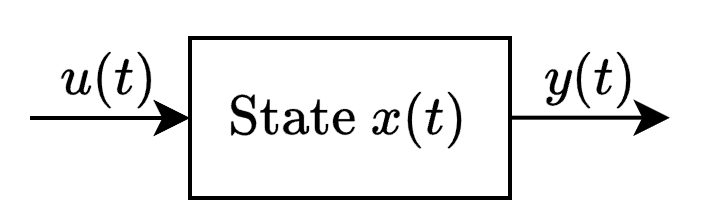
\includegraphics[width=0.4\linewidth]{images/rep.png}
\end{figure}

\subsection{State space representation}
State space (or internal) representation describes a system where the state $\mathbf{x}(t)$ comprises internal variables known as states. 
The system can be represented as:
\[\begin{cases}
    \mathbf{x}(t+1)=\mathbf{Fx}(t)+\mathbf{G}u(t) \\
    y(t)=\mathbf{Hx}(t)+\mathbf{D}u(t)
\end{cases}\]
Here, $\mathbf{x}(t+1)=\mathbf{Fx}(t)+\mathbf{G}u(t)$ is termed the state equation, a difference equation, and $y(t)=\mathbf{Hx}(t)+\mathbf{D}u(t)$ is the output equation.
In the case of a single input single output system, $\mathbf{F}$ (state matrix) is an $n \times n$ matrix, $\mathbf{G}$ (input matrix) is an $n \times 1$ column vector, $\mathbf{H}$ (output matrix) is a $1 \times n$ row vector, and $\mathbf{D}$ (input-output matrix) is a scalar. 
\begin{definition}[\textit{Strictly proper system}]
    A system is termed strictly proper if the input doesn't directly affect the output.
\end{definition}
\begin{property}
    The system is strictly proper if the matrix $\mathbf{D}$ is zero. 
\end{property}    
\begin{property}
    The system is stable if the eigenvalues of the matrix $\mathbf{F}$ lie within the unit circle.
\end{property}
The state space representation of the system is not unique. 
We can transform it as follows:
\[\begin{cases}
    \mathbf{F}^\prime = \mathbf{TFT}^{-1} \\ 
    \mathbf{G}^\prime = \mathbf{TG} \\
    \mathbf{H}^\prime = \mathbf{HT}^{-1} \\ 
    \mathbf{D}^\prime = \mathbf{D}
\end{cases}\]
These representations are equivalent for all invertible square matrices $ \mathbf{T}$, where $ \mathbf{T}$ is an $n \times n$ matrix.

\subsection{Transfer function representation}
The transfer function (or external) representation is derived from the input/output time domain difference equation by utilizing the delay operator $z^{-1}$: 
\[z^{-1} \mathbf{x}(t)= \mathbf{x}(t-1) \qquad z^{1}\mathbf{x}(t)=\mathbf{x}(t+1)\]
\noindent In general we have: 
\begin{figure}[H]
    \centering
    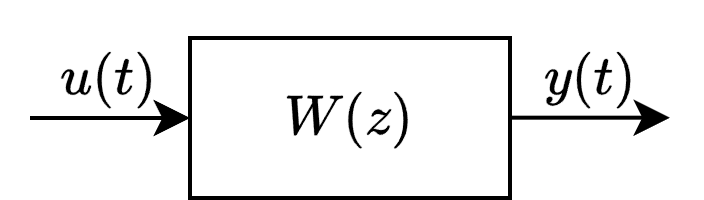
\includegraphics[width=0.4\linewidth]{images/transfer.png}
\end{figure}
\noindent In general, the transfer function can be represented as:
\[W(z)=\dfrac{B(z)}{A(z)}z^{-k}=\dfrac{b_0+b_1 z^{-1}+\cdots+b_p z^{-p}}{a_0+a_1 z^{-1}+\cdots+a_n z^{-n}}z^{-k}\]
\begin{property}
    The system is strictly proper if the time delay $k$ is greater than or equal to one.
\end{property}    

\subsection{Impulse response representation}
This representation, also known as convolution of the input with the impulse response, relies on the impulse in discrete time, which has a value of one at time zero and null values at all other instants.

The response of the system at successive instants starting from zero constitutes the impulse response $\omega(t)$: 
\[\text{impulse response}=\left\{ \omega(0),\omega(1),\omega(2),\omega(3),\dots \right\}\]
The output of the system can be expressed as:
\[y(t)=\sum_{k=0}^{+\infty}\omega(k)u(t-k)\]
Thus, the output $y(t)$ is the convolution of the generic input signal $u(t)$ with the impulse response coefficients.

\paragraph*{Filters}
The filter: 
\[W(z)=\dfrac{z^{-1}+\frac{1}{2}z^{-2}}{1+\frac{1}{3}z^{-1}}\]
is termed an Infinite Impulse Response filter.

The filter: 
\[W(z)=z^{-1}+\dfrac{1}{2}z^{-2}+\dfrac{1}{3}z^{-3}\]
is referred to as a Finite Impulse Response filter.